\section*{Problem 3}
	\begin{proof} [Solution]
		We can expect the barcode as following:
		\begin{itemize}
			\item At first, there are total 8 points. Thus start with 8 0th dimension.
			\item After some time has passed, since all points have the same distance, they are connected at the same time. Thus 7 points will be dead(note that one 0th dimension is still left) and one 1st dimension complex will be created at that time.
		\end{itemize}
		To check this, plot the result by using Python.
		\begin{center}
			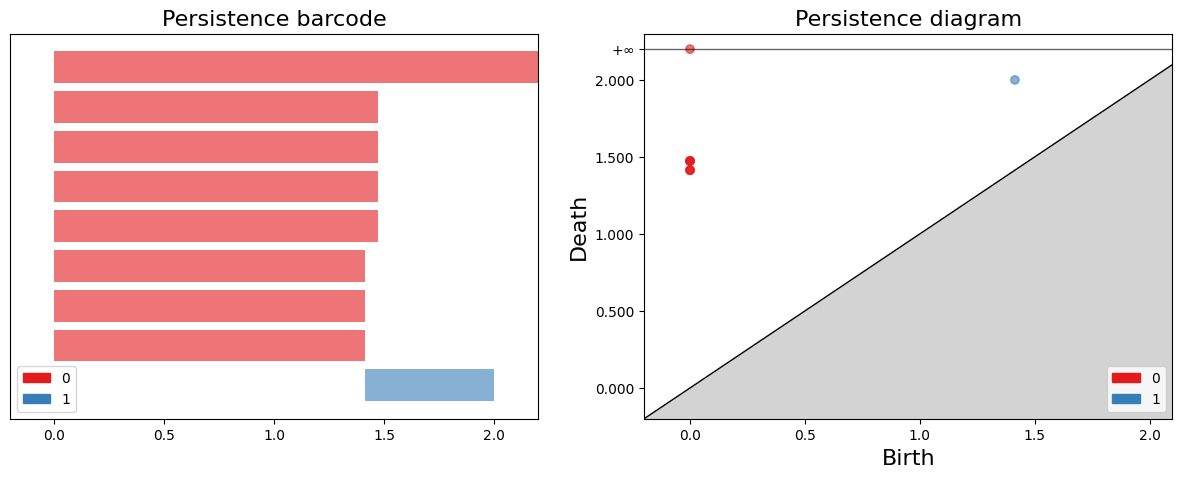
\includegraphics[width=\textwidth]{persis.png}
		\end{center}
	\end{proof}